\section{\textbf{Disjoint-Output AGI-Former}}

The disjoint-output architecture is the first end-to-end AGI-Former organization. It preserves a separate perception-to-action branch for each supported modality while sharing the causal history of prior thoughts and actions. This design is appropriate when output spaces have different vocabularies, temporal resolutions, physical meanings, or execution constraints. For example, a language response, a motor command, a visual generation token, and an audio-control token need not be forced into one output head merely because they occur within the same agent.

Figure~\ref{fig:agi_former_disjoint} shows the architecture. Image patches, video tubelets, audio waveform or spectrogram tokens, and text or other sensory embeddings are processed by modality-specific Unified MHA encoders. During training, previous action tokens are processed by a causal Unified MHA encoder-in-decoder. Its output supplies a shared thought--action state to every modality branch. Each Unified X-MHA decoder then conditions that state on one encoded modality and produces a distinct action-token stream.

\begin{figure*}[t]
    \centering
    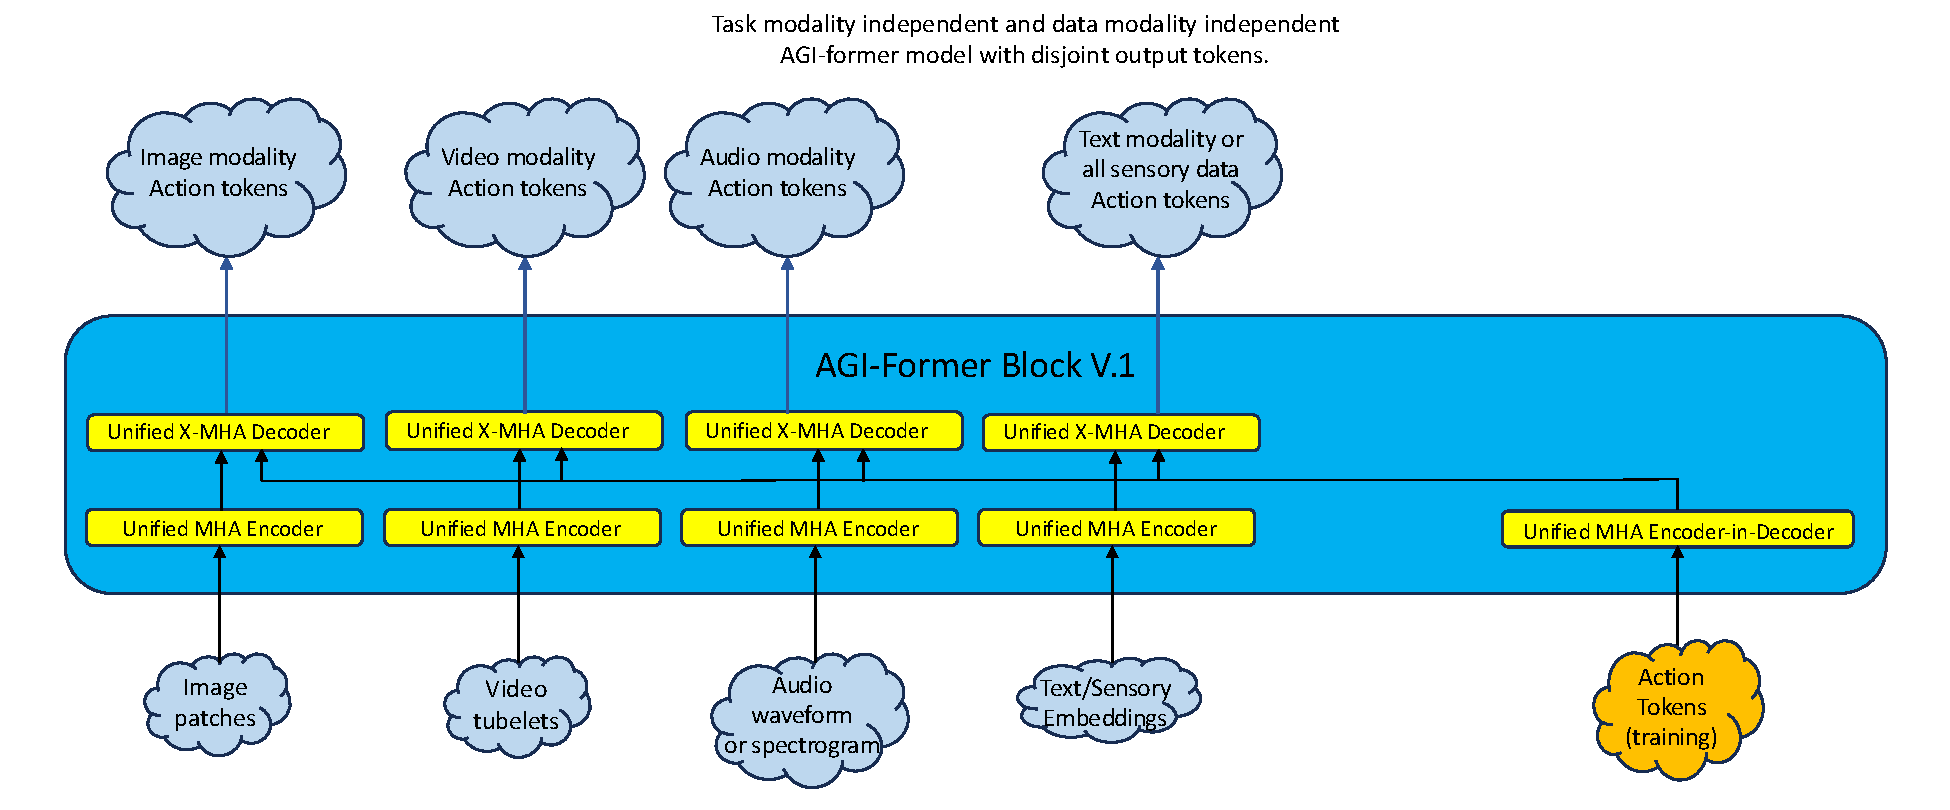
\includegraphics[width=\textwidth]{Figures/fig2.pdf}
    \caption{Disjoint-output AGI-Former. Modality-native inputs are encoded independently, while a shared causal thought--action state conditions one Unified Cross-MHA decoder per modality. Each branch retains a separate output-token space. Ground-truth history is supplied during teacher-forced training; generated history is used autoregressively during inference.}
    \label{fig:agi_former_disjoint}
\end{figure*}

\subsection{\textbf{Unified Modality Encoders}}

Let $\mathcal{M}_{\mathrm{out}}\subseteq\mathcal{M}$ denote the modalities associated with disjoint output branches. Following the notation of Section~III, the token sequence $X_t^{(m)}$ is projected into the common model dimension and encoded as

\begin{equation}
\begin{aligned}
    H_t^{(m)}
    &= \operatorname{UMHAEnc}_{m}\!\left(
       X_t^{(m)};\theta_{E_m}
       \right)
     \in\mathbb{R}^{N_{m,t}\times d},
    &&m\in\mathcal{M}_{\mathrm{out}}.
\end{aligned}
\label{eq:disjoint_modality_encoder}
\end{equation}

Here, $\operatorname{UMHAEnc}_{m}$ denotes a stack of modality-specific Unified MHA encoder blocks derived from the unified-attention formulation of UTR \cite{zohourian2026utr}. The encoders need not share parameters or sequence lengths. Their common output width $d$ defines the interface through which the action state can attend to any branch.

For a missing modality, no synthetic observation is required. Let $r_t^{(m)}\in\{0,1\}$ indicate whether modality $m$ is available at step $t$. The active encoded set is

\begin{equation}
\begin{aligned}
    \mathcal{H}_t
    &= \left\{
       H_t^{(m)}:
       m\in\mathcal{M}_{\mathrm{out}},\;
       r_t^{(m)}=1
       \right\}.
\end{aligned}
\label{eq:active_modalities}
\end{equation}

This definition permits asynchronous sensors and modality dropout without changing the parameterization of the remaining branches.

\subsection{\textbf{Shared Causal Thought--Action State}}

The architecture uses one causal state to condition all disjoint branches. During teacher-forced training, let $\widetilde{Y}_{<t}$ denote the ground-truth thought--action history shifted by one token. During inference, let $\widehat{Y}_{<t}$ contain the tokens generated by the model. The history supplied to the encoder-in-decoder is therefore

\begin{equation}
\begin{aligned}
    Y^{\star}_{<t}
    &=
    \begin{cases}
        \widetilde{Y}_{<t}, & \text{training},\\
        \widehat{Y}_{<t},   & \text{inference},
    \end{cases}\\
    S_t
    &= \operatorname{UMHAED}\!\left(
       Y^{\star}_{<t};\theta_{A}
       \right)
     \in\mathbb{R}^{L_{<t}\times d},
\end{aligned}
\label{eq:disjoint_action_state}
\end{equation}

where $\operatorname{UMHAED}$ is the masked Unified MHA encoder-in-decoder shown in Fig.~\ref{fig:agi_former_disjoint}. The causal mask prevents a position from accessing future thought or action tokens.

Because the branches generate different streams, their completed outputs must be represented consistently in the next decision history. Let $\rho$ be a deterministic serialization operator that inserts branch identifiers, temporal markers, and termination tokens before interleaving or concatenating the outputs:

\begin{equation}
\begin{aligned}
    Y_t
    &= \rho\!\left(
       \left\{y_t^{(m)}\right\}_{m\in\mathcal{M}_{\mathrm{out}}}
       \right),\\
    Y_{<t+1}
    &= \left[Y_{<t};Y_t\right].
\end{aligned}
\label{eq:disjoint_history_update}
\end{equation}

The operator $\rho$ does not fuse branch representations. It only records what each branch produced so that later decisions can be conditioned on the complete prior behavior of the agent.

\subsection{\textbf{Per-Modality Unified Cross-Attention}}

For each available modality, a Unified X-MHA decoder uses the causal state as the decoding stream and the modality encoding as its conditioning stream. We denote the branch output by

\begin{equation}
\begin{aligned}
    Z_t^{(m)}
    &= \operatorname{UXMHADec}_{m}\!\left(
       S_t,H_t^{(m)};\theta_{D_m}
       \right)
     \in\mathbb{R}^{L_t^{(m)}\times d},\\
    &\hspace{7.2cm}
       m\in\mathcal{M}_{\mathrm{out}},\;r_t^{(m)}=1.
\end{aligned}
\label{eq:disjoint_cross_attention}
\end{equation}

The ordering of the arguments is significant: $S_t$ determines the current decision context, and $H_t^{(m)}$ supplies the modality-native evidence relevant to that context. The Unified X-MHA operation is independently parameterized for each branch unless parameter sharing is imposed as an experimental constraint. This independence allows image, video, audio, language, and actuator branches to learn different attention patterns while receiving the same causal history.

Residual and feedforward processing at branch $m$ and layer $\ell$ can be written as

\begin{equation}
\begin{aligned}
    C_{t,\ell}^{(m)}
    &= \operatorname{LN}\!\left(
       S_{t,\ell}^{(m)}+
       \operatorname{UXMHA}_{m,\ell}\!\left(
       S_{t,\ell}^{(m)},H_t^{(m)}
       \right)
       \right),\\
    S_{t,\ell+1}^{(m)}
    &= \operatorname{LN}\!\left(
       C_{t,\ell}^{(m)}+
       \operatorname{FFN}_{m,\ell}\!\left(C_{t,\ell}^{(m)}\right)
       \right).
\end{aligned}
\label{eq:disjoint_decoder_layer}
\end{equation}

Equation~\eqref{eq:disjoint_decoder_layer} specifies the branch interface without constraining the internal unified-attention parameterization, which follows UTR and can be varied through ablation.

\subsection{\textbf{Independent Output Heads and Training Objective}}

Each branch maps its decoder representation to its own output space $\mathcal{V}_m$. For discrete action tokens,

\begin{equation}
\begin{aligned}
    P_t^{(m)}
    &= \operatorname{softmax}\!\left(
       Z_t^{(m)}W_{O}^{(m)}+b_{O}^{(m)}
       \right),\\
    \widehat{y}_{t,j}^{(m)}
    &\sim P_t^{(m)}[j,:],
    &&j=1,\ldots,L_t^{(m)}.
\end{aligned}
\label{eq:disjoint_output_head}
\end{equation}

Continuous actions may instead be represented by quantized tokens or predicted through a distributional regression head. Keeping $W_O^{(m)}$ branch specific avoids requiring semantically unrelated outputs to share a vocabulary.

Let $q_t^{(m)}\in\{0,1\}$ indicate that a target output is available for branch $m$ at step $t$. The multi-branch training objective is

\begin{equation}
\begin{aligned}
    \mathcal{L}_{\mathrm{dis}}
    &= \sum_{m\in\mathcal{M}_{\mathrm{out}}}
       \lambda_m
       \sum_{t=1}^{T}q_t^{(m)}
       \mathcal{L}_{m,t},\\
    \mathcal{L}_{m,t}
    &= -\sum_{j=1}^{L_t^{(m)}}
       \log P_t^{(m)}
       \!\left[j,y_{t,j}^{(m)}\right],\\
    \lambda_m&\geq0,
    \qquad
    \sum_{m\in\mathcal{M}_{\mathrm{out}}}\lambda_m=1.
\end{aligned}
\label{eq:disjoint_loss}
\end{equation}

The weights $\lambda_m$ prevent branches with longer sequences or denser supervision from dominating optimization. They may be fixed, uncertainty weighted, or adapted according to gradient balance. When the encoders and causal-state module are trainable, gradients from every supervised branch update the shared perception--state--action system, while each output head retains its own semantics.

\subsection{\textbf{Inference and Branch Coordination}}

At inference, all active branches can decode in parallel after $S_t$ and their respective $H_t^{(m)}$ have been computed. A branch terminates when it produces its end token or satisfies an actuator-specific stopping rule. If simultaneous outputs are permitted, the environment executes the resulting set. If outputs compete for one resource, a deterministic safety or scheduling policy $\Pi$ selects an executable subset:

\begin{equation}
\begin{aligned}
    \widehat{\mathcal{Y}}_t^{\mathrm{dis}}
    &= \left\{
       \widehat{y}_t^{(m)}:
       m\in\mathcal{M}_{\mathrm{out}},\;r_t^{(m)}=1
       \right\},\\
    \mathcal{E}_t
    &= \Pi\!\left(
       \widehat{\mathcal{Y}}_t^{\mathrm{dis}},c_t
       \right),
\end{aligned}
\label{eq:disjoint_execution}
\end{equation}

where $c_t$ contains environmental constraints, permissions, and safety rules. The policy $\Pi$ is not a substitute for learned joint reasoning; it prevents incompatible commands from being executed when the architecture intentionally retains disjoint outputs.

\subsection{\textbf{Capabilities and Limitations}}

The disjoint architecture provides four practical advantages. First, it accommodates heterogeneous output spaces without a universal action vocabulary. Second, branches can be trained with partially labeled datasets because $q_t^{(m)}$ masks unavailable targets. Third, branch-specific representations and heads make modality-level errors easier to isolate. Fourth, independent branches can be added or replaced without retraining every output projection, although changes to shared components may still require joint adaptation.

Its central limitation is the absence of a final learned fusion stage. Branches share prior history but do not directly negotiate their current outputs before generation. Conflicts may therefore be resolved only at the next autoregressive step or by the execution policy $\Pi$. Computation also grows with the number and length of active branches, and independently optimized losses can generate negative transfer through shared components. These limitations motivate the joint-output architecture in Section~V, where action-conditioned modality representations are combined before the final action sequence is generated.
